\section{Architecture Design}


\begin{figure}[H]
    \centering
    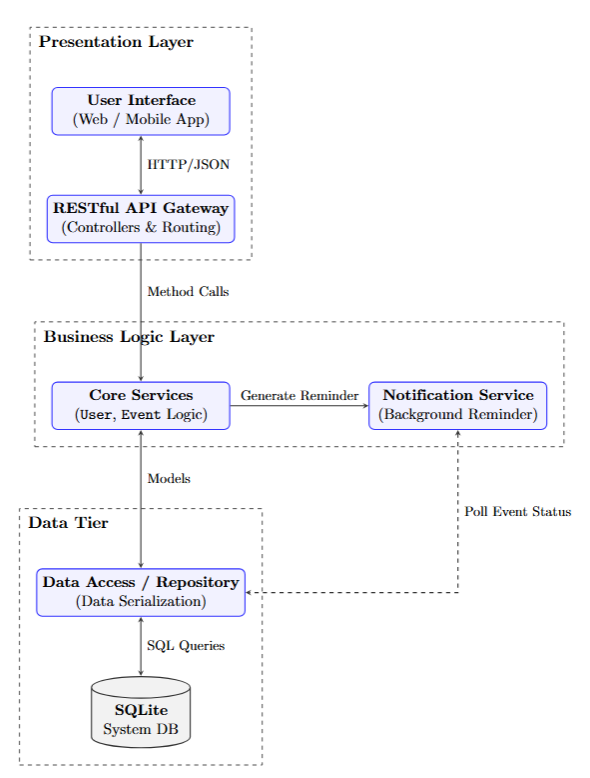
\includegraphics[width=0.75\textwidth]{pictures/archi.png}
    \caption{Sơ đồ Kiến trúc phân tầng của hệ thống SERS}
\end{figure}



\subsection{Các thành phần và Đáp ứng NFR1}
\begin{enumerate}[leftmargin=*]
    \item \textbf{Presentation Layer (Tầng Giao diện):} Nhận thao tác từ người dùng và chuyển tiếp xuống hệ thống (tương ứng với mũi tên "Gửi yêu cầu" trong Hình 1 và 2).
    \item \textbf{Business Logic Layer (Tầng Nghiệp vụ):} Dựa theo Class Diagram (Hình 4), tầng này chứa:
    \begin{itemize}
        \item \textbf{Core Services (\texttt{User}, \texttt{Event}):} Chịu trách nhiệm thực thi các CRUD logic, kiểm tra dữ liệu hợp lệ và chuyển đổi các trạng thái (\texttt{EventStatus}).
        \item \textbf{Notification Service (Đáp ứng NFR1):} Để đảm bảo thông báo gửi trong vòng 60 giây (NFR1), class \texttt{NotificationService} được chạy như một tiến trình ngầm (Background Service). Nó thực thi hàm \texttt{checkPendingReminders()} liên tục truy vấn Data Tier (với chu kỳ quét ngắn khoảng 30s) để \texttt{triggerReminder()} kịp thời.
    \end{itemize}
    \item \textbf{Data Tier (Tầng Dữ liệu):} Lưu trữ toàn bộ thông tin của Hệ thống quản lý SERS, trả kết quả truy vấn ("Xác nhận lưu thành công", "Xác nhận xóa thành công") lên tầng nghiệp vụ.
\end{enumerate}

\subsection{Đề xuất Công nghệ sử dụng}
\begin{itemize}[leftmargin=*]
    \item \textbf{Backend:} \textbf{FastAPI (Python)}. Khung làm việc này nhẹ, hỗ trợ xử lý bất đồng bộ (async), rất phù hợp để hiện thực hóa các class trong Hình 4.
    \item \textbf{Background Task:} \textbf{APScheduler}. Công cụ hoàn hảo để chạy class \texttt{NotificationService} ngầm dưới nền, đáp ứng việc check thời gian liên tục mà không làm chậm các API tạo/sửa sự kiện.
    \item \textbf{Database:} \textbf{SQLite}. Tích hợp sẵn trong Python, đủ mạnh để lưu trữ dữ liệu dự án môn học.
\end{itemize}
